\section{Implementazioni utilizzate}
In questa tesi vengono messe a confronto due configurazioni diverse di leggi di contollo che condividono l'algoritmo di trajectory planning. La gestione del percorso non è trattata, vengono definiti per effettuare le simulazione una sequesza di punti nello spazio accompagnati dal tempo alla quale la posizione specifica deve essere raggiunta.
Uno schema generale della configurazione del software dell'autopilota è riportato nella Figura (\ref{fig:Autopilota}).


\begin{figure}
	\centering
	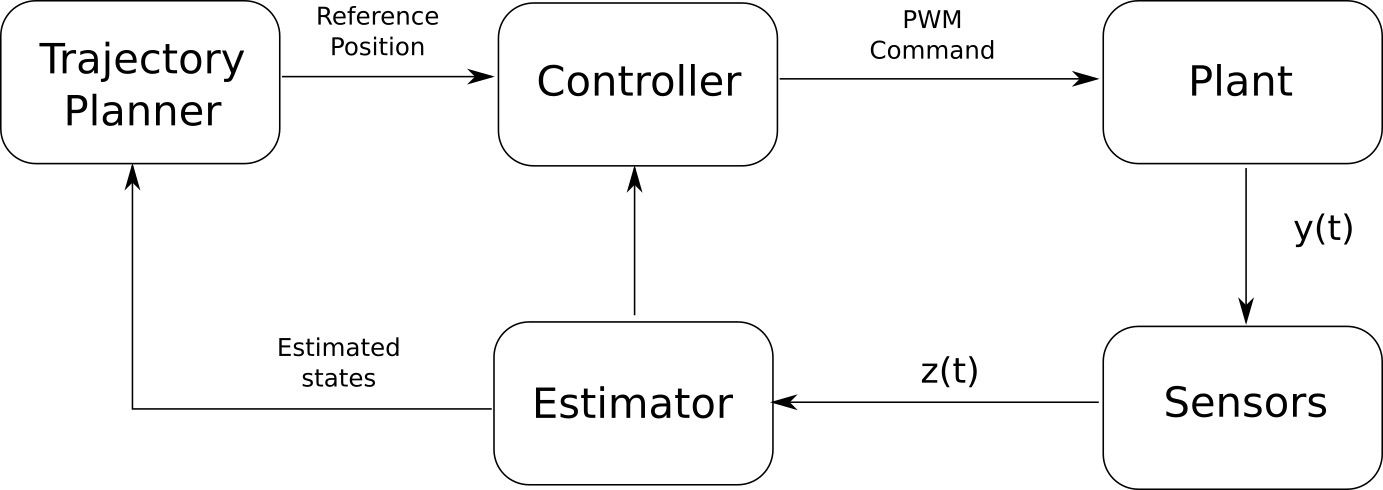
\includegraphics[width=0.6\textwidth]{SistemaQuadrirotore/Figure/Autopilota}
	\caption{Schema della configurazione dell'autopilota}
	\label{fig:Autopilota}
\end{figure}

L'algoritmo implementato per generare la traiettoria è uguale per tutti i tipi di simulazioni che sono state fatte. Data una sequenza di punti espressi in termini di coordinate nello spazio e il tempo rispetto all'inizio della simulazione per raggiungimento di tale punto, viene definita una legge della traiettoria con profilo di velocità a forma trapezoidale, utilizzando come vincolo la velocità massima posta a $g/2$, \cite{DesTestCarm}.

Sia nelle simulazioni MIL e SIL due tipologie di controllori vengono messi a confronto. In entrambe le configurazioni il controllore viene suddiviso in tre componenti base: Altitude Controller, Attitude Controller e Position Controller, come mostrato in Figura (\ref{fig:Controller}).

Da questo momento si farà riferimento alla denominazione di controllore PID nel caso in cui i tre controllori siano derivati da controllori PID, mentre si parlerà di controllore SMC, nell'implementazione in sui compare il controllore SMC nel modulo di Altitude e di Attitude.

\begin{figure}
	\centering
	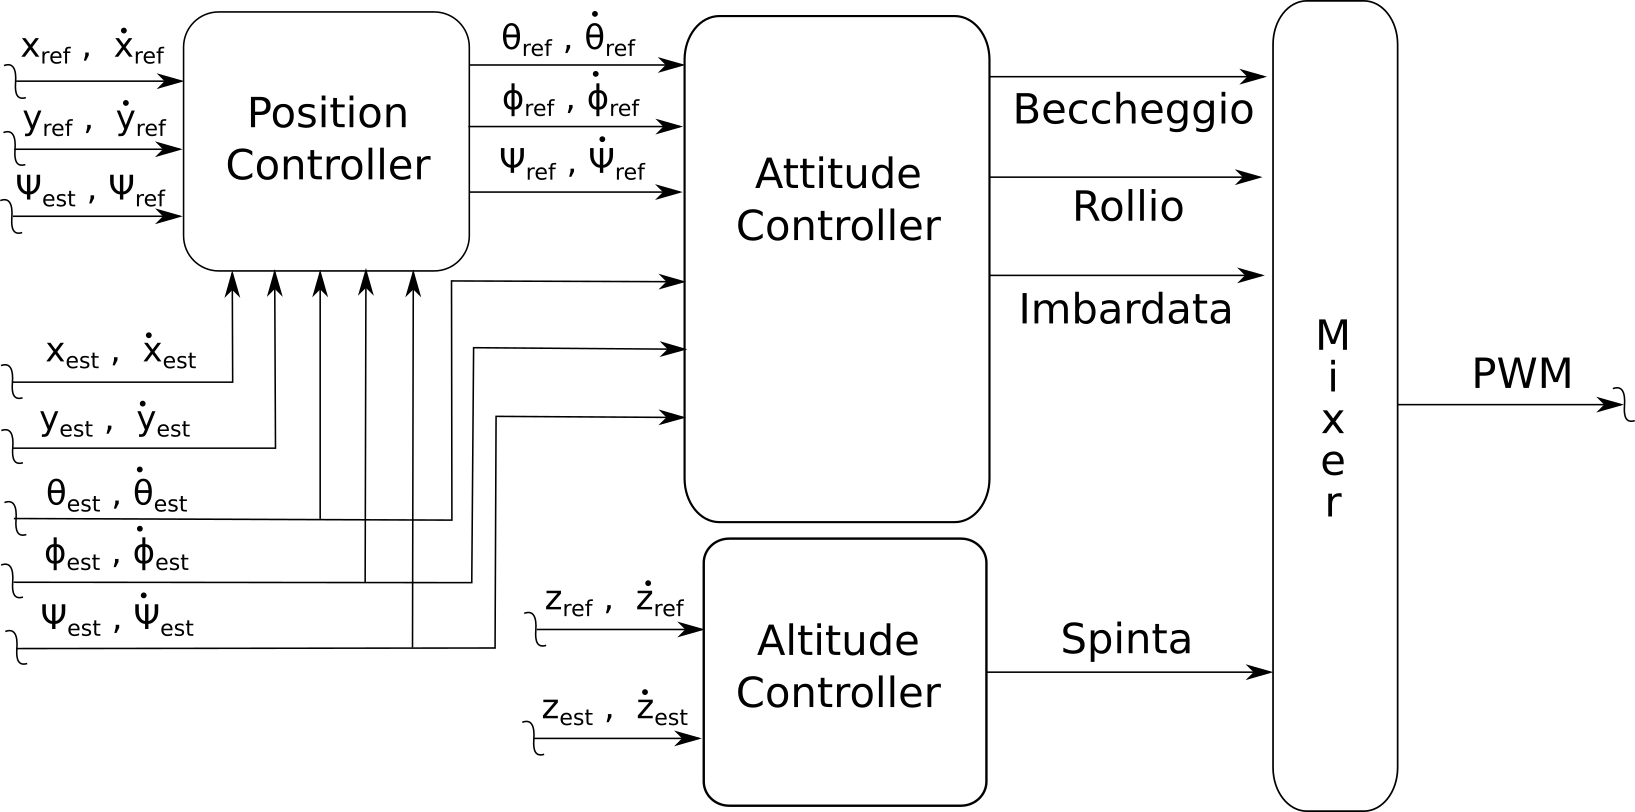
\includegraphics[width=0.7\textwidth]{SistemaQuadrirotore/Figure/Controllore}
	\caption{Schema della configurazione del software dell'autopilota}
	\label{fig:Controller}
\end{figure}

Il primo tipo di controllore implementa il modulo di Attitude Control come mostrato in Figura (\ref{fig:PIDAttitudeCTR}). In questo modello si utilizza una versione modificata del PID, dove il contributo derivativo è determinato dalla misura dei ratei angolari sugli assetti. I parametri utilizzati sono riassunti nella Tabella (\ref{tab:PIDATT}).

\begin{figure}
	\centering
	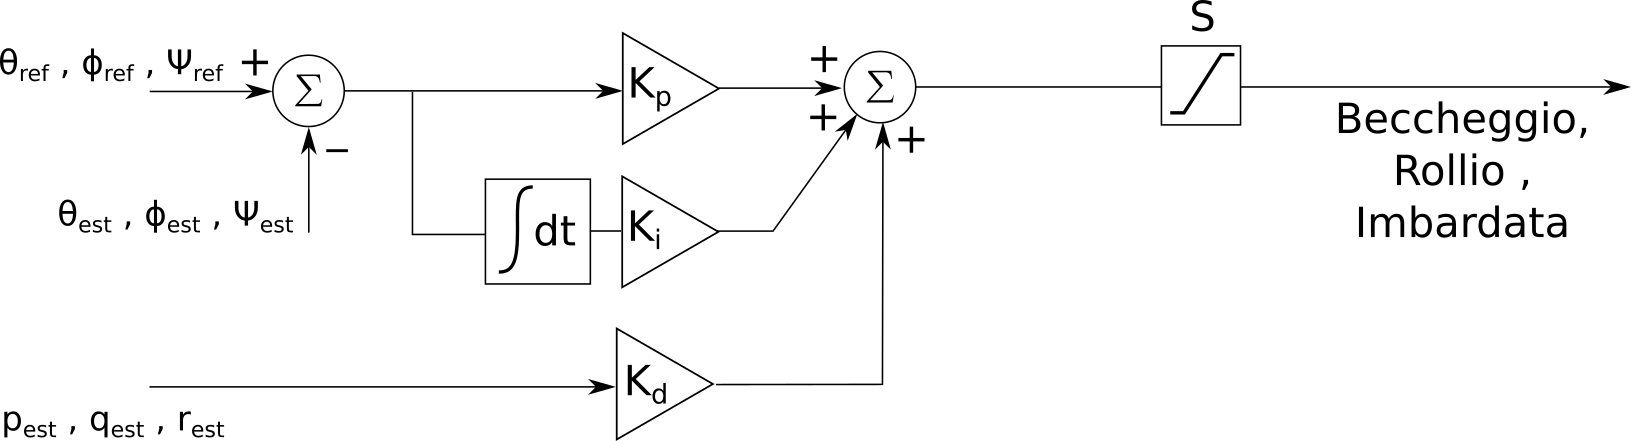
\includegraphics[width=0.7\textwidth]{SistemaQuadrirotore/Figure/PIDAttitudeCtrl}
	\caption{Schema del Attitude Controller}
	\label{fig:PIDAttitudeCTR}
\end{figure}


\begin{table}
	\centering
	\begin{tabular}{c c c}
		\hline
		Canale  & Parametro & Valore \\
		\hline
		\multirow{4}{*}{Beccheggio / Rollio}&$K_p$ & 0.531 \\
		&$K_d$ & 0.031\\
		&$K_i$ & -0.156\\
		&$S$ & -1 $\leftrightarrow$ 1\\
		\hline
		\multirow{4}{*}{Imbardata}&$K_p$ & 5 \\
		&$K_d$ & 1\\
		&$K_i$ & -1\\
		&$S$ & -1 $\leftrightarrow$ 1\\
		\hline
	\end{tabular}	
	\caption{Parametri PID - Attitude Controller}
	\label{tab:PIDATT}
\end{table}

Nel modello del Altitude Controller, Figura (\ref{fig:PIDAltitudeCTR}), viene implementato un controllore PID con contributo derivativo ricavato dalla misura di errore relativa al rateo di salita/discesa. I parametri utilizzati sono riuassunti in Tabella (\ref{tab:PIDALT}).

\begin{figure}
	\centering
	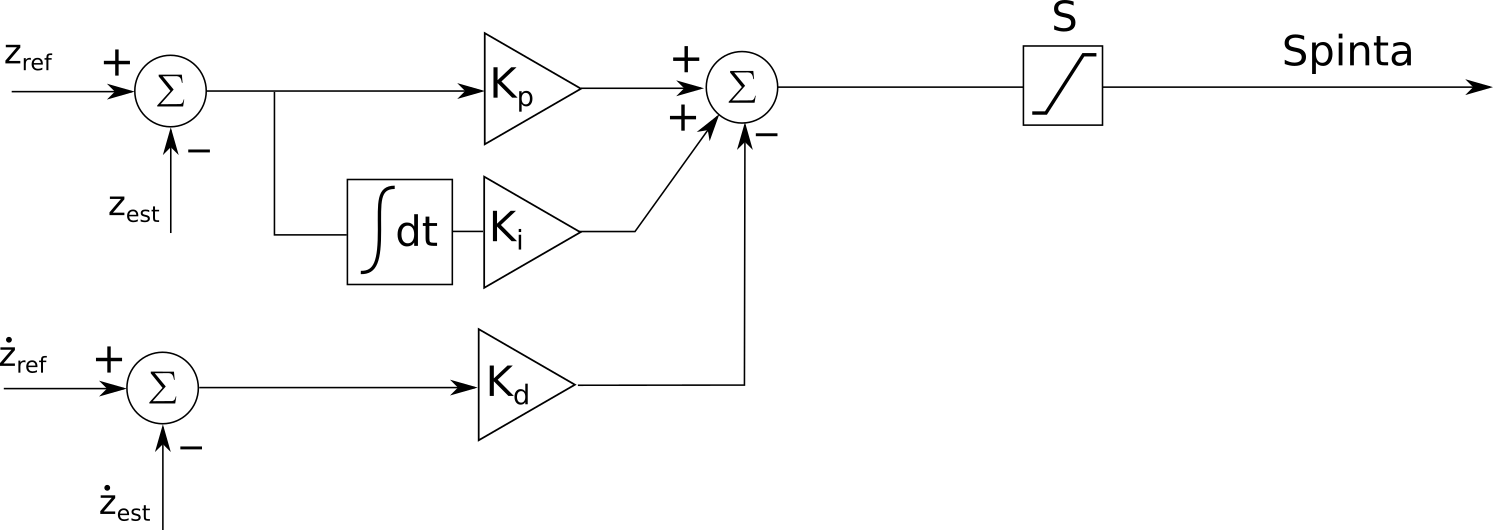
\includegraphics[width=0.7\textwidth]{SistemaQuadrirotore/Figure/PIDAltitudeCtrl}
	\caption{Schema del Altidude Controller}
	\label{fig:PIDAltitudeCTR}
\end{figure}

\begin{table}
	\centering
	\begin{tabular}{c c}
		\hline
		Parametro & Valore \\
		\hline
		$K_p$ & -1.875 \\
		$K_d$ & -1.188\\
		$K_i$ & 0.625\\
		$S$ & 0 $\leftrightarrow$ 1\\
		\hline
	\end{tabular}	
	\caption{Parametri PID - Altitude Controller}
	\label{tab:PIDALT}
\end{table}

Nell'ultimo modello relativo al Position Controller, Figura (\ref{fig:PIDPosCTR}), viene implementata una configurazione di PID particolare. In questo modello, per ridurre l'overshot sulla posizione, si introduce un contributo derivativo proporzionale alla derivata dell'errore sulla velocità $K_{dd}$, \cite{DesTestCarm}. Nella Tabella (\ref{tab:PIDPOS}), vengono riassunti i parametri utilizzati per le simulazioni. 

\begin{figure}
	\centering
	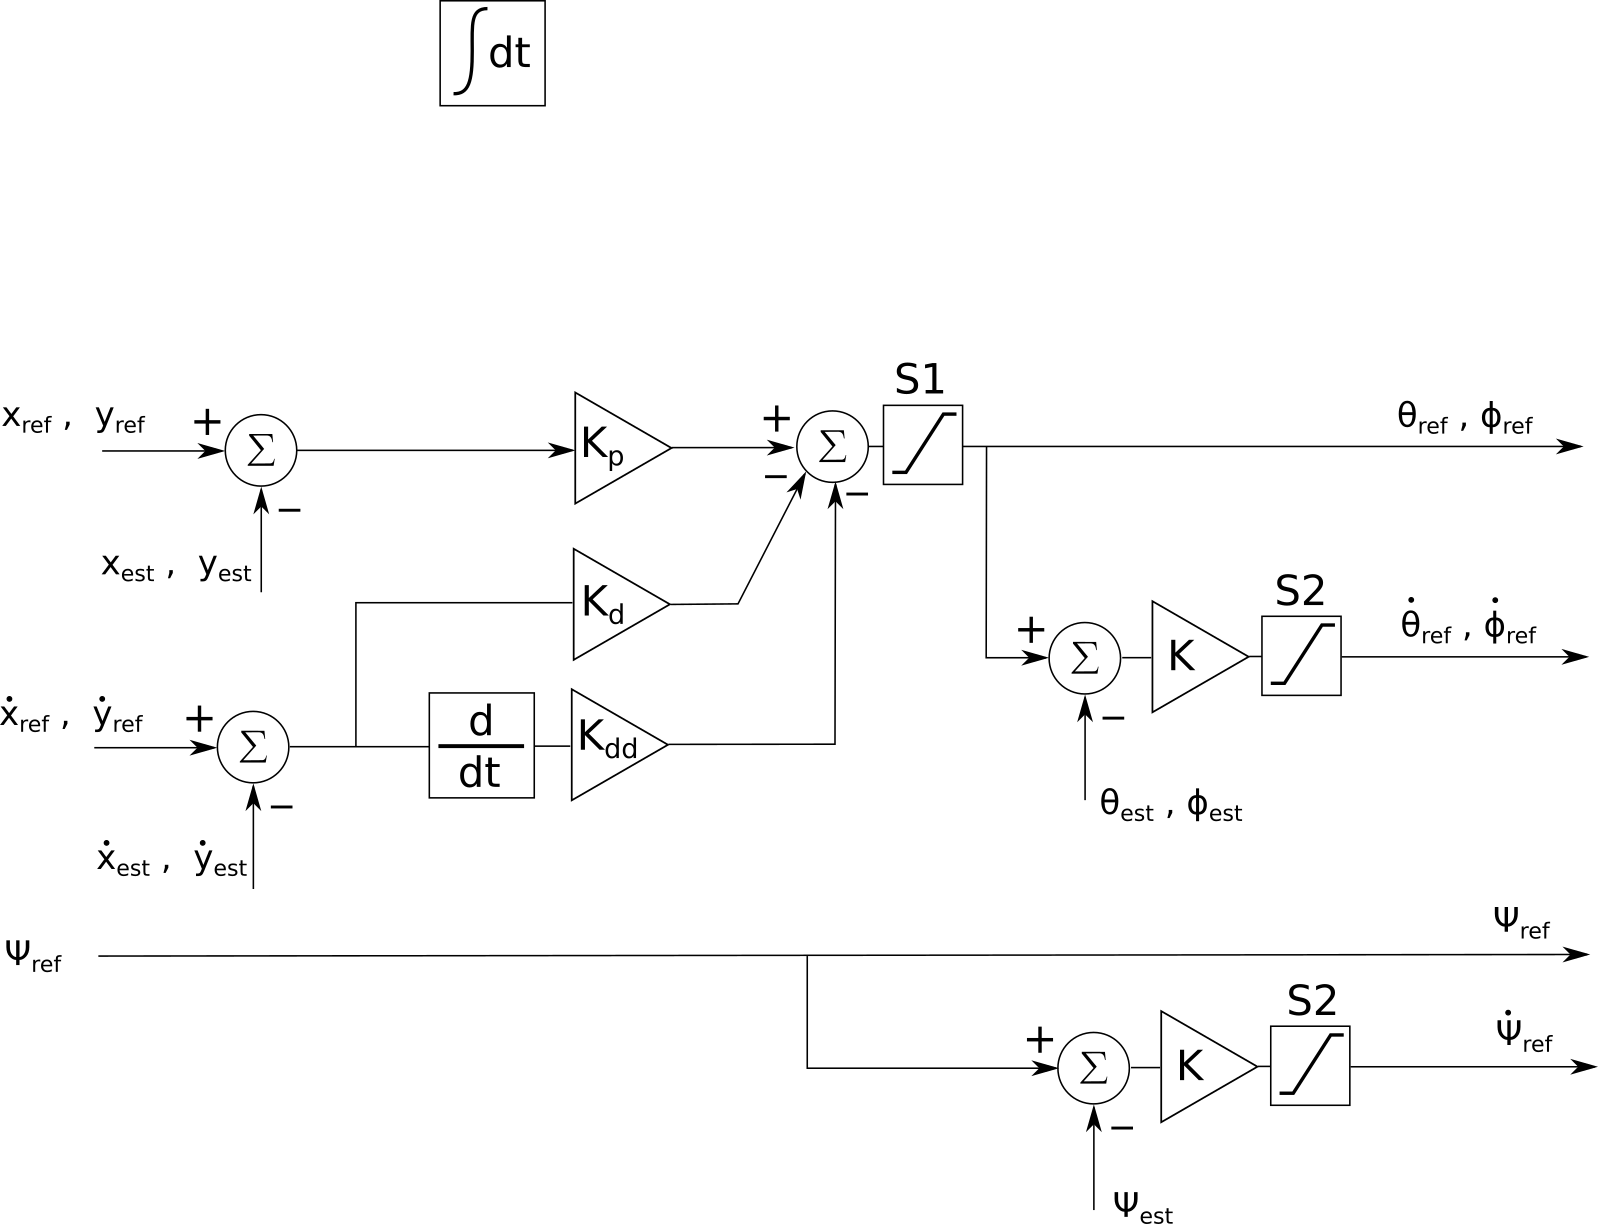
\includegraphics[width=0.7\textwidth]{SistemaQuadrirotore/Figure/PIDPositionCtrl}
	\caption{Schema del Position Controller}
	\label{fig:PIDPosCTR}
\end{figure}

\begin{table}
	\centering
	\begin{tabular}{c c c}
		\hline
		 Canale & Parametro & Valore \\
		\hline
		\multirow{3}{*}{$\theta$}&$K_p$ & -1.5 \\
		&$K_d$ & 1.5\\
		&$K_{dd}$ & 0.3\\
		\hline
		\multirow{3}{*}{$\phi$}& $K_p$ & 1.5 \\
		&$K_d$ & -1.5\\
		&$K_{dd}$ & -0,3\\
		\hline
		\multirow{3}{*}{$\theta$, $\phi$}&$K$ & 2 \\ 
		&$S1$ & -0.524 [rad] $\leftrightarrow$ +0.524 [rad]\\
		&$S2$ & -1 [rad/s] $\leftrightarrow$ 1  [rad/s]\\
		\hline
		\multirow{2}{*}{$\psi$}&$K$ & 2 \\
		&$S3$ & -0.5 [rad/s] $\leftrightarrow$ 0.5 [rad/s]\\
		\hline
		
	\end{tabular}	
	\caption{Parametri PID - Position Controller}
	\label{tab:PIDPOS}
\end{table}

Nel secondo sistema di controllo simulato, denominato SMC, il modulo di Position Control è identico come configurazione al la versione PID ma con parametri riportati in Tabella (\ref{tab:SMCPOS}), di fatto rimuovendo il contributo della derivata dell'errore misurato rispetto alle velocità, $K_{dd}$.

\begin{table}
	\centering
	\begin{tabular}{c c c}
		\hline
		Canale & Parametro & Valore \\
		\hline
		\multirow{3}{*}{$\theta$}&$K_p$ & -1.5 \\
		&$K_d$ & 0.5\\
		&$K_{dd}$ & 0\\
		\hline
		\multirow{3}{*}{$\phi$}& $K_p$ & 1.5 \\
		&$K_d$ & -0.5\\
		&$K_{dd}$ & 0\\
		\hline
		\multirow{3}{*}{$\theta$, $\phi$}&$K$ & 2 \\ 
		&$S1$ & -0.524 [rad] $\leftrightarrow$ +0.524 [rad]\\
		&$S2$ & -1 [rad/s] $\leftrightarrow$ 1  [rad/s]\\
		\hline
		\multirow{2}{*}{$\psi$}&$K$ & 2 \\
		&$S3$ & -0.5 [rad/s] $\leftrightarrow$ 0.5 [rad/s]\\
		\hline		
	\end{tabular}	
	\caption{Parametri SMC - Position Controller}
	\label{tab:SMCPOS}
\end{table}

La leggi di controllo nell'applicazione con SMC derivano dalla scrittura delle derivate seconde della dinamica, Eq. (\ref{eq:SistemaQuadrirotore_hdd}).
\begin{equation}\label{eq:SistemaQuadrirotore_hdd}
\begin{array}{r@{}l}
	\ddot{h} = & g -\cos(\theta)\cos(\phi)\frac{F_z}{m} \\[1ex]
	\ddot{\phi} = &\frac{J_y -J_z}{J_x} \dot{\theta} \dot{\psi} + \frac{\tau_x}{J_x} \\[1ex]
	\ddot{\theta}  = & \frac{J_z -J_x}{J_y} \dot{\phi} \dot{\psi} + \frac{\tau_y}{J_y} \\[1ex]
	\ddot{\psi}  = & \frac{J_x -J_y}{J_z} \dot{\theta} \dot{\phi} + \frac{\tau_z}{J_z} 
\end{array}
\end{equation}

Per il sistema di Altitude control viene scelta una superficie definita nell'equazione (\ref{eq:SistemaQuadrirotore_s_h}).
\begin{equation}\label{eq:SistemaQuadrirotore_s_h}
	s(z) = \dot{z}_{ref} - \dot{z}_{est} + \lambda (z_{ref} - z_{est})
\end{equation}

Da questa scelta, nel rispetto della condizione (\ref{eq:SistemaQuadrirotore_SMC_cond}) e supponendo che la derivata seconda di $s$ sia nulla, si ottiene la legge di controllo espressa nella formula (\ref{eq:SistemaQuadrirotore_HCTRL}).

\begin{equation}\label{eq:SistemaQuadrirotore_HCTRL}
	F_z = -\frac{m}{\cos(\phi) \cos(\theta)} (\lambda (\dot{z}_{ref}-\dot{z}_{est})- g) - K \textit{sign}(s(z))
\end{equation}

Nella Figura (\ref{fig:SMC_ALT}), è presentato lo schema di controllo applicato nel modello . I parametri utilizzati sono riassunti nella Tabella (\ref{tab:ab:SMC_ALT}).

\begin{figure}
	\centering
	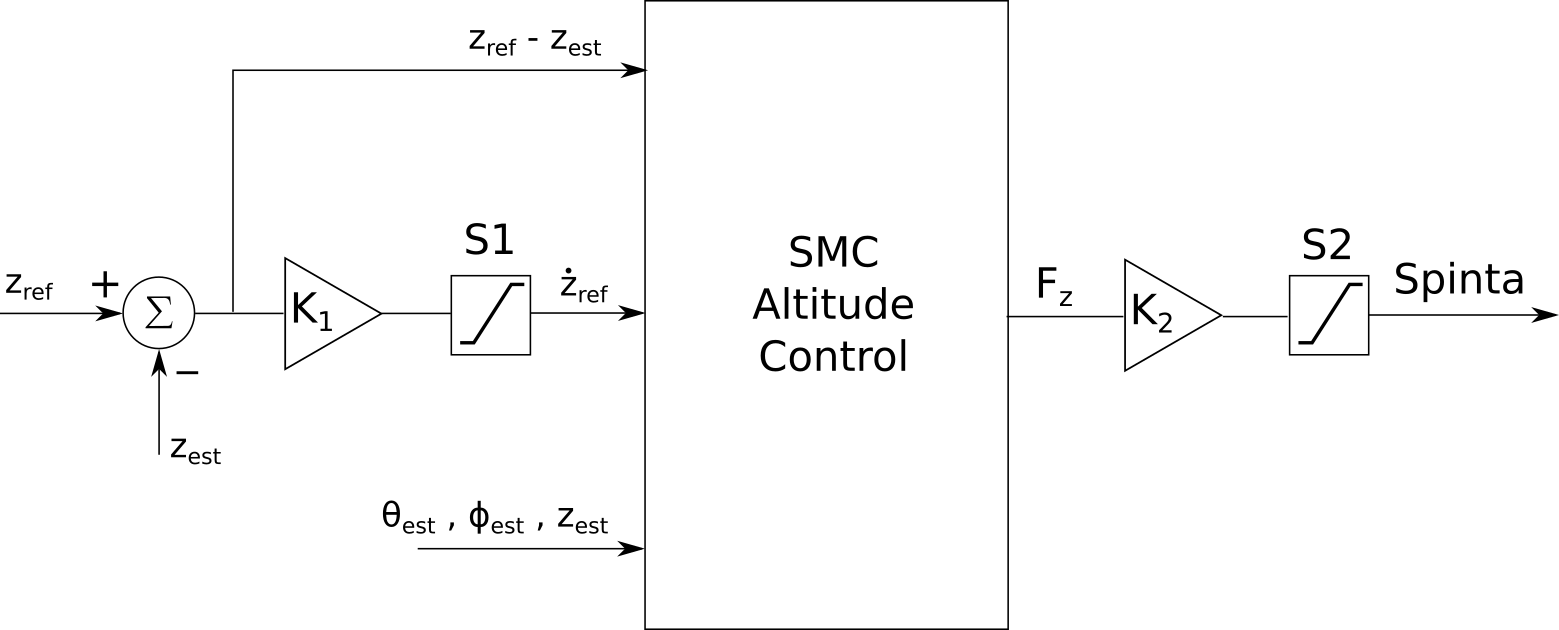
\includegraphics[width=0.7\textwidth]{SistemaQuadrirotore/Figure/SMCAltitudeCtrl}
	\caption{Schema del Altidude Controller utilizzando il controllo SMC}
	\label{fig:SMC_ALT}
\end{figure}

\begin{table}
	\centering
	\begin{tabular}{c c}
		\hline
		Parametro & Valore \\
		\hline
		$K_1$ & 10 \\
		$K_2$ & 0.0313\\
		$K$ & 4\\
		$\lambda$ & 20\\
		$S1$ & -10 $\leftrightarrow$ +10\\
		$S2$ & 0 $\leftrightarrow$ 1\\
		\hline
	\end{tabular}	
	\caption{Parametri SMC - Altitude Controller}
	\label{tab:ab:SMC_ALT}
\end{table}

Analogamente per il sistema di Altitude Control, nel sistema di Attitude Control viene scelta una superficie di sliding espressa dall'equazione (\ref{eq:SistemaQuadrirotore_slideATT}), utilizzando la definizione di $\mathfrak{q}_{err}$ riportata nella formula (\ref{eq:SistemaQuadrirotore_errore}), \cite{DesTestCarm}.

\begin{equation}\label{eq:SistemaQuadrirotore_slideATT}
	s(\phi, \theta, \psi, \mathbf{q}_{err}) =  \begin{Bmatrix}
		\dot{\phi}_{ref} - \dot{\phi}_{est} \\
		\dot{\theta}_{ref} - \dot{\theta}_{est} \\
		\dot{\psi}_{ref} - \dot{\psi}_{est} \\
	\end{Bmatrix} + \begin{pmatrix}
		\lambda_{roll} & 0 & 0 \\
		0 & \lambda_{pitch} & 0 \\
		0 & 0 & \lambda_{yaw} \\
	\end{pmatrix} \mathbf{q}_{err}
\end{equation}

Dove $\mathbf{q}_{err}$ è la parte immaginaria del quaternione $\mathfrak{q}_{err}$.

Determinando la derivata prima di $s$ e ponendo la derivata seconda di $s$ nulla, imponendo la condizione (\ref{eq:SistemaQuadrirotore_SMC_cond}) si ottiene infine la legge di controllo, Eq. (\ref{eq:SistemaQuadrirotore_SMCATT}), \cite{DesTestCarm}.

\begin{equation}\label{eq:SistemaQuadrirotore_SMCATT}
\begin{Bmatrix}
\tau_x \\ \tau_y \\ \tau_z 
\end{Bmatrix} = - \begin{Bmatrix}
	(J_y -J_z)\dot{\psi} \dot{\theta} \\
	(J_z -J_x)\dot{\psi} \dot{\phi} \\
	(J_x -J_y)\dot{\theta} \dot{\phi} \\
\end{Bmatrix} +
	\Lambda
	\begin{pmatrix}
	J_x & 0 & 0 \\
	0 & J_y & 0 \\
	0 & 0 & J_z \\
	\end{pmatrix}
	\mathbf{q}_{err} 
	-
	K
	\textit{sign}(s)
\end{equation}

Dove 
\[
\Lambda = 
\begin{pmatrix}
\lambda_{roll} & 0 & 0 \\
0 & \lambda_{pitch} & 0 \\
0 & 0 & \lambda_{yaw} \\
\end{pmatrix} \ , \ 
K = \begin{pmatrix}
K_{roll} & 0 & 0 \\
0 & K_{pitch} & 0 \\
0 & 0 & K_{yaw} \\	
\end{pmatrix}
\]

Nella Figura (\ref{fig:SMC_ATT}), è presentato lo schema di controllo applicato nel modello. I parametri utilizzati sono riassunti nella Tabella (\ref{tab:ab:SMC_ATT}).

\begin{figure}
	\centering
	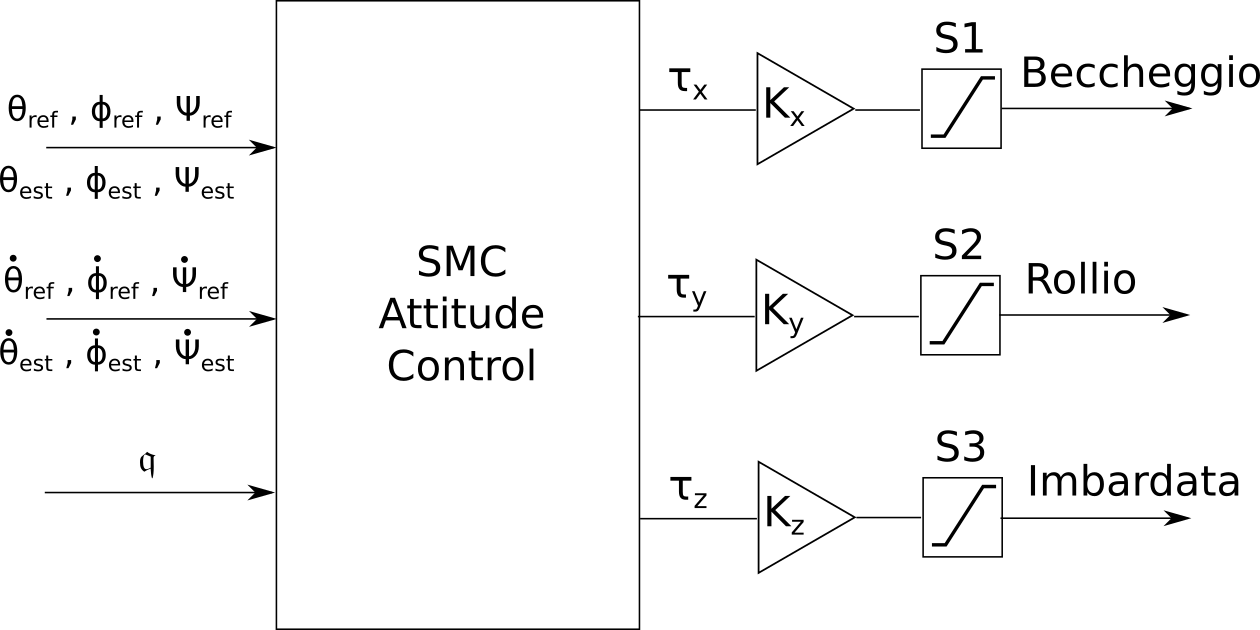
\includegraphics[width=0.7\textwidth]{SistemaQuadrirotore/Figure/SMCAttitudeCtrl}
	\caption{Schema del Attidude Controller utilizzando il controllo SMC}
	\label{fig:SMC_ATT}
\end{figure}

\begin{table}
	\centering
	\begin{tabular}{c c c}
		\hline
		Canale  & Parametro & Valore \\
		\hline
		\multirow{4}{*}{Beccheggio}&$K_x$ & 0.313 [1/Nm]\\
		&$K_{pitch}$ & -0.25\\
		&$\lambda_{pitch}$ & 20\\
		&$S1$ & -1 $\leftrightarrow$ 1\\
		\hline
		\multirow{4}{*}{Rollio}&$K_y$ & 0.313 [1/Nm]\\
		&$K_{roll}$ & -0.25\\
		&$\lambda_{roll}$ & 20\\
		&$S2$ & -1 $\leftrightarrow$ 1\\
		\hline
		\multirow{4}{*}{Imbardata}&$K_z$ & 1 [1/Nm]\\
		&$K_{yaw}$ & -0.25\\
		&$\lambda_{yaw}$ & 10\\
		&$S3$ & -1 $\leftrightarrow$ 1\\
		\hline
	\end{tabular}	
	\caption{Parametri SMC - Attitude Controller}
	\label{tab:ab:SMC_ATT}
\end{table}
\clearpage
In uscita dai tre moduli di controllo sopracitati quindi ci sono quattro segnali :
\begin{itemize}
	\item \textbf{Spinta:} Comando $T$ definito da 0 a 1
	\item \textbf{Imbardata:} Comando $Y$ definito da -1 a 1
	\item \textbf{Rollio:} Comando $R$ definito da -1 a 1
	\item \textbf{Beccheggio:} Comando $P$ definito da -1 a 1
\end{itemize}

Il modulo Mixer si occupa di determinare a partire da questi segnali il comando espresso in termini di Duty Cycle (DC), per generare il segnale elettrico utilizzando la Power-Width Modulation (PWM), in modo da comunicare con il componente che aziona l'attuatore, ovvero l'Electronic Speed Controller (ESC), \cite{DesTestCarm}. Seguendo la descrizione della guida presente in rete del Firmware PX4 si può definire la legge matematica che descrive il mixer, Eq. (\ref{eq:SistemaQuadrirotore_MIXER}).

\begin{equation}\label{eq:SistemaQuadrirotore_MIXER}
	\begin{array}{r@{}l}
		\nu_1 = & \left(\frac{-R +P +Y}{2} + T\right) 1000 + 1000 \\[1ex]
		\nu_2 = & \left(\frac{R -P +Y}{2} + T\right) 1000 + 1000 \\[1ex]
		\nu_3 = & \left(\frac{R +P -Y}{2} + T\right) 1000 + 1000 \\[1ex]
		\nu_4 = & \left(\frac{-R -P -Y}{2} + T\right) 1000 + 1000 \\[1ex]
	\end{array}
\end{equation}
